%------------------
% General Settings
%------------------
\def \docTitle      {Data sheet}
\def \docSubTitle   {M101}
\def \productNumber {M101}
\def \productName   {Rotation Stage}
\def \docAuthor     {LK-Instruments}
\def \docRevision   {Rev. 001}
\def \docSubject    {\docAuthor \docTitle \docSubTitle}
\def \docKeywords   {\docAuthor, \productName, \productNumber, SMC2242, SMC4242}

\documentclass[a4paper, final, 12pt, oneside]{scrartcl}

%----------
% Packages
%----------
\usepackage{etex}
\reserveinserts{30}
\usepackage[utf8]{inputenc}
%\usepackage[latin1]{inputenc} % erlaubt Umlaute in der tex-Datei

\usepackage{slantsc}
\usepackage[urw-garamond]{mathdesign}
\usepackage{garamondx}
\usepackage[T1]{fontenc}

\usepackage[english]{babel}              % For the hyphenations in different languages
\usepackage[intlimits]{amsmath}          % math symbols
\usepackage{braket}                      % Dirac braket notation
\usepackage{graphicx}                    % include pictures
\usepackage{color}
\usepackage[shell]{gnuplottex}           % gnuplot in latex
\usepackage{pstricks}                    % post script tricks
\usepackage{listings}                    % enter programming code
\usepackage{fancyhdr}                    % make quite nice header/footer
\usepackage[version=3]{mhchem}           % chemistry stuff
\usepackage{relsize}
\usepackage{afterpage}
\usepackage{gensymb}
\usepackage{textcomp}
\usepackage{multicol}
%\usepackage{subfig}
\usepackage{lipsum}
\usepackage{multirow,booktabs,colortbl,tabularx}
\usepackage{caption}
\usepackage{subcaption}


\usepackage{pgfplots}
\usepackage{tikz}                        % beautiful plots
\pgfplotsset{compat = newest}
\usepackage{units}                       % easy to use number-unit-package
\usepackage[section]{placeins}           % Float barrier for sections.


\usepackage{listings}					% erlaubt Quellcode mit Zeilenumbruechen

%----------------
% PDF properties
%----------------
\usepackage[
  pdftitle={\docAuthor~\docSubTitle~\docTitle}
 ,pdfsubject={\docSubject}
 ,pdfauthor={\docAuthor}
 ,pdfkeywords={\docKeywords}
 ,pdfcreator={\docAuthor}
 ,pdfstartview=Fit                       % startseite ganz anzeigen
 ,pdfborder={0 0 0}                      % links ohne umrandungen
 ,pdfdisplaydoctitle=true                % pdftitle statt dateinamen anzeigen
 ,pdfcenterwindow=true                   % position pdf in center of the screen
 ,setpagesize=true
]{hyperref}

%-------------------
% Header und Footer
%-------------------
\fancyhf{}        % clear all header/footer
\renewcommand{\headrulewidth}{0pt}
%\renewcommand{\sectionmark}[1]{\markboth{#1}{}}
%\renewcommand{\subsectionmark}[1]{\markright{#1}}
\fancyhead[RE,RO]{\productNumber}
\fancyfoot[LE,LO]{\docAuthor}
\fancyfoot[CE,CO]{\docRevision}
\fancyfoot[RE,RO]{\thepage}

\pagestyle{fancy}

% number equations with sections before equation-index
\numberwithin{equation}{section}
\numberwithin{table}{section}
\numberwithin{figure}{section}

%---------------------
% My code definitions
%---------------------

\newtheorem{envdefinition}{Definition}[section]
\newtheorem{envsatz}{Satz}

% special numbers and letters
\renewcommand{\i}{\mathrm{i}}                  % complex i
\newcommand{\e}{\mathrm{e}}                    % Eulers number
\renewcommand{\phi}{\varphi}                   % nicer phi
\renewcommand{\epsilon}{\varepsilon}           % nicer epsilon
\renewcommand{\theta}{\vartheta}               % nicer theta
\renewcommand{\rho}{\varrho}                   % nicer rho
%\newcommand{\degree}{^{\circ}}                 % degree-circle

% vectors and matrices
\renewcommand{\vec}[1]{\boldsymbol{#1}}
\newcommand{\Vek}[3]{\left(\begin{array}{c}#1\\#2 
\ifthenelse{\equal{#3}{}}{}{\\#3}\end{array}\right)}

% integral and derivative stuff:
\renewcommand{\d}[1]{\;\mathrm{d}#1}           % integeration d
% total derivative
\newcommand{\td}[1]{\frac{\mathrm{d}}{\mathrm{d}#1}\,}
\newcommand{\pd}[1]{\partial_{#1}\,}             % partial derivative

% Braket notation
\renewcommand{\bra}{\Bra}
\renewcommand{\ket}{\Ket}
\renewcommand{\braket}{\Braket}
\renewcommand{\set}{\Set}

% plus-minus with braces
\newcommand{\PM}{\ensuremath{\substack{+\\[-0.25em]-}\,}}
\renewcommand{\pm}{\PM}
\newcommand{\pmp}{\ensuremath{\substack{\mathsmaller{(}+\mathsmaller{)}\\[-0.25em]-}\,}}
\newcommand{\pmm}{\ensuremath{\substack{+\\[-0.25em]\mathsmaller{(}-\mathsmaller{)}}\,}}

\setlength{\columnsep}{40.0pt}

%----------------------------------------------------------
% let the party start
%----------------------------------------------------------
\begin{document}
\thispagestyle{empty}

\includegraphics[width=0.1\textwidth]{../general/logo_black.pdf}
\hfill {\Huge \textbf{\textsf{\productName}}} \hfill {\Huge \textbf{\textsf{\productNumber}}}\\
\noindent\rule{\textwidth}{0.4pt}

\begin{multicols}{2}
\subsection*{Features}
\begin{itemize}
  \item[] Hall-sensor controlled automatic zero-positioning
  \item[] Standard SM1-compatible mount for optical elements
  \item[] Angular resolution $\leq 0.01^{\circ}$
  \item[] Low backlash $\leq 0.1^{\circ}$
\end{itemize}
\FloatBarrier

\subsection*{Applications}
\begin{itemize}
  \item[] Mirror positioning
  \item[] Polarization adjustment
  \item[] Grating positioning
  \item[] Neutral density filter positioning
\end{itemize}
\FloatBarrier

\subsection*{Description}
The LK-Instruments M101 is a robust and ball bearing mounted rotation
stage designed for carrying optical elements. It can be mounted to the
experimental setup from any axis with standard M6 screws, headless screws,
posts and post holders. 
\end{multicols}
\noindent\rule{\textwidth}{0.4pt}
\vspace*{0.5cm}

\centerline{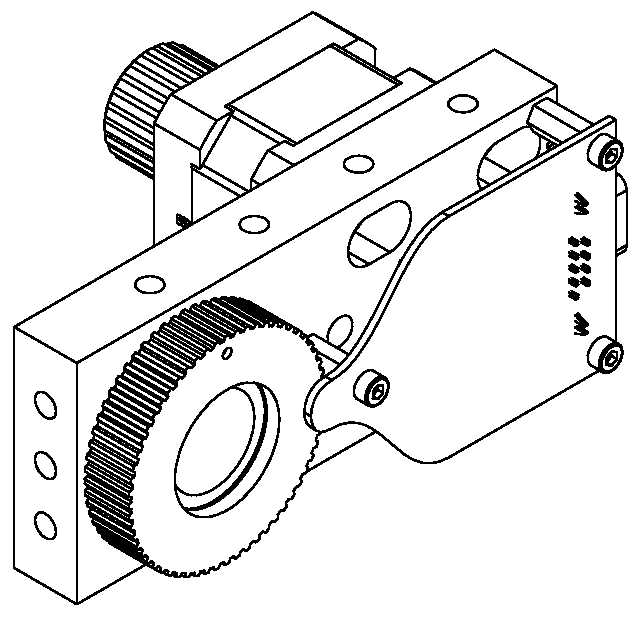
\includegraphics[width=0.6\textwidth]{./drawings/m101_full_dwg.pdf}}

\vfill
\begin{minipage}{\textwidth}
  \begin{minipage}[t]{0.49\textwidth}
      
    
  \end{minipage}
  \hfill
  \begin{minipage}[t]{0.49\textwidth}
    \begin{flushright}
    {\footnotesize LK-Instruments\\
             Unterbrüdener Str. 14\\
             71549 Auenwald\\
             Germany\\
             \href{http://www.lk-instruments.com}{www.lk-instruments.com}}
    \end{flushright}
  \end{minipage}
\end{minipage}






\FloatBarrier

\newpage
\subsection*{Specifications}
$T_A = \unit[25]{^{\circ}C}$ and 50\% RH unless otherwise noticed.
\newcolumntype{C}[1]{>{\centering\arraybackslash}p{#1}}
\begin{table}[!htp]
  \centering
  \begin{tabular}{C{2cm} C{2cm} *{3}{C{1cm}} *{3}{C{1cm}} C{1.5cm} }
    \toprule
    \textbf{Parameter} & \textbf{Conditions} &
    \multicolumn{3}{p{3cm}}{\centering\textbf{M101A}} &
    \multicolumn{3}{p{3cm}}{\centering\textbf{M101B}} &
    \textbf{Unit} \\
    \cmidrule(lr){3-5} \cmidrule(lr){6-8}
    & &
    Min & Typ & Max &
    Min & Typ & Max &\\
    \midrule
    Current &  & 0.1 & 1.3 & 1.33 & 0.1 & 1.65 & 1.68 & A/Phase\\ \midrule
    Holding torque & Microst.=1, Curr.=1.33A & & 66 & & & 132 & & Ncm \\ \midrule
    Step angle & Microst.=1 & & 0.3 & & & 0.3 & & deg \\ \midrule
    Step angle accuracy &  & & 1.7 & & & 1.7 & & \% \\ \midrule
    Backlash &  & & 0.1 & & & 0.1 & & deg \\ \midrule
    Gear ratio &  & & 3 & & & 3 & &  \\ \midrule
    Velocity & Microst.=1, 2 ms/step & & 150 & & & 150 & & deg/s \\ \midrule
    Load capacity & radial/axial & &  & 5/2.5 & &  & 5/2.5 & kg \\ \midrule
    Weight &  & & 0.504 & & & 0.634 & & kg \\ \midrule
    Temperature range &  & -10 &  & 50 & -10 &  & 50 & $^{\circ}$C \\
    \bottomrule
  \end{tabular}
\end{table}
\vfill
\paragraph{Microstepping.} A physical property of stepper motors is that the holding
torque decreases heavily with the amount of adjusted microsteps. For the M101A
and M101B rotation stages the decrease is shown in the diagrams below.
\begin{figure}[!hbp]
\centering
  \begin{subfigure}{.5\textwidth}
    \centering
    \caption*{M101A}
    \begin{tikzpicture}
    \begin{axis}
      [
        height = 0.65\textwidth,
        width  = \textwidth,  
        xmin = 0.7,
        xmax = 48,
        xtick={1,2,4,8,16,32},
        xticklabels={1,2,4,8,16,32},
        xlabel = Microsteps,
        ymin = 0,
        ymax = 70,
        % yticklabels={},
        ylabel = Ncm,
        xmode = log,
        log basis x={2}
      ]
  
      \pgfplotstableread{holding_torque.csv} \datatableA
  
      \addplot [mark=+, only marks,
               % error bars/.cd,
               % x dir=none,
               % y dir=both, y explicit
               ]
        table[x=substeps, y=m101a] from \datatableA;
    \end{axis}
  \end{tikzpicture}
  \end{subfigure}%
  \begin{subfigure}{.5\textwidth}
    \centering
    \caption*{M101B}
    \begin{tikzpicture}
    \begin{axis}
      [
        height = 0.65\textwidth,
        width  = \textwidth,  
        xmin = 0.7,
        xmax = 48,
        xtick={1,2,4,8,16,32},
        xticklabels={1,2,4,8,16,32},
        xlabel = Microsteps,
        ymin = 0,
        ymax = 140,
        % yticklabels={},
        ylabel = Ncm,
        xmode = log,
        log basis x={2}
      ]
  
      \pgfplotstableread{holding_torque.csv} \datatableB
  
      \addplot [mark=+, only marks,
               % error bars/.cd,
               % x dir=none,
               % y dir=both, y explicit
               ]
        table[x=substeps, y=m101b] from \datatableB;
    \end{axis}
  \end{tikzpicture}
  \end{subfigure}
  \label{fig:test}
\end{figure}
\FloatBarrier

\subsection*{Outline Dimensions}
All dimensions in millimeters.
\begin{figure}[!htp]
  \centering
  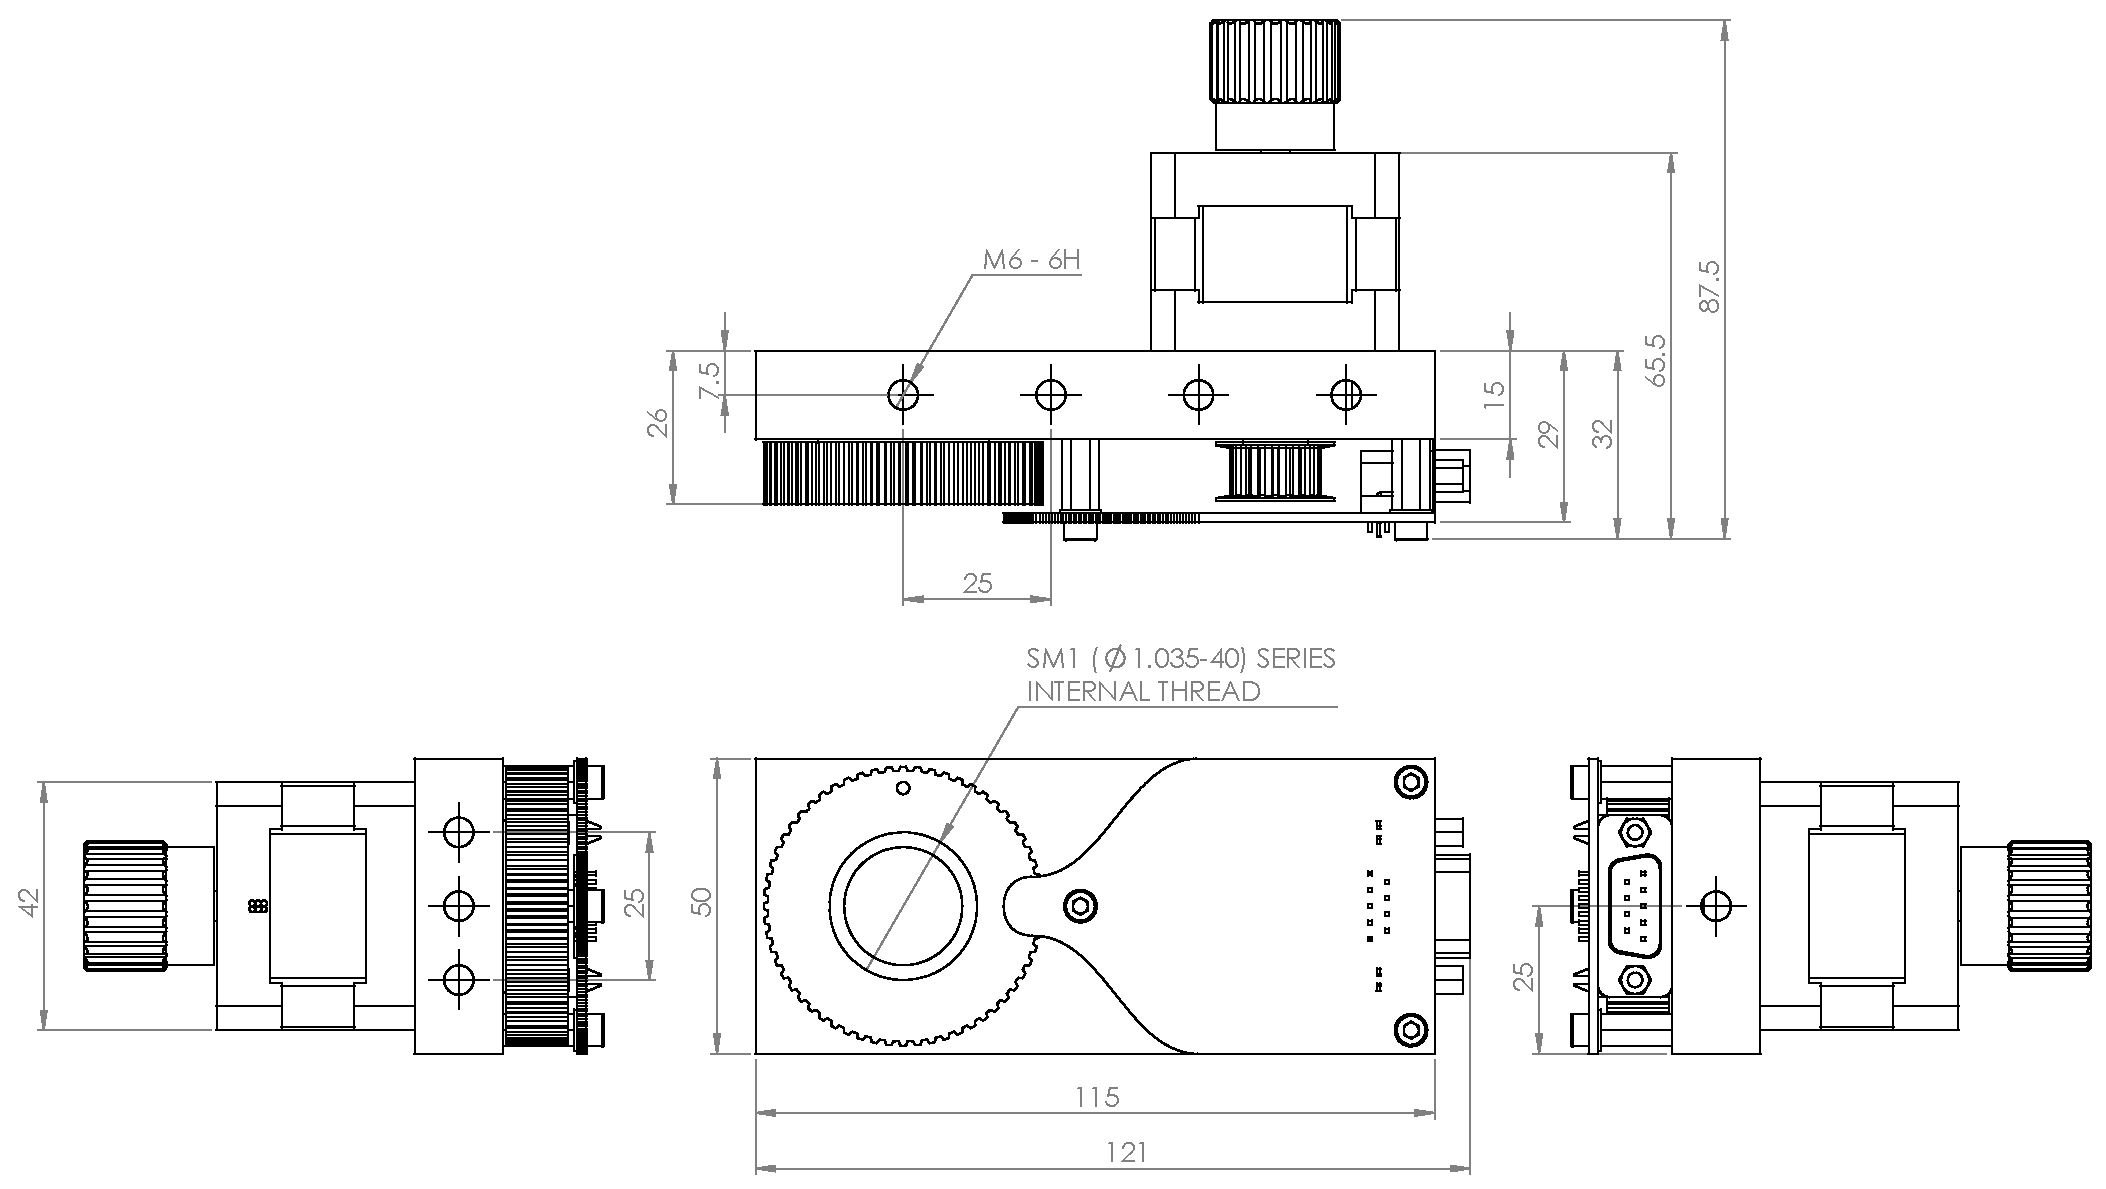
\includegraphics[angle=0,origin=c,width=0.7\textwidth]{./drawings/M101_outline_dimensions.pdf}
\end{figure}
%\vfill
\FloatBarrier

\subsection*{Pin Configuration}
\begin{minipage}{\textwidth}
  \begin{minipage}[b]{0.49\textwidth}
    \centering
    D-SUB-9 female connector\\
    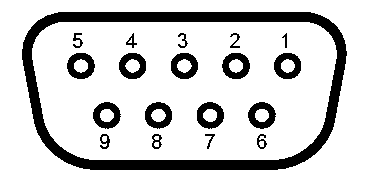
\includegraphics[width=0.6\textwidth]{./drawings/Numbered_DE9_female_Diagram.pdf}\\
    Front view
  \end{minipage}
  \hfill
  \begin{minipage}[b]{0.49\textwidth}
    \centering
    \begin{tabular}{cc}
      \toprule
      \textbf{Pin} & \textbf{Function} \\
      \toprule
      1 & Phase B1 \\ \midrule
      2 & Phase B2\\ \midrule
      3 & Phase A2 \\ \midrule
      4 & Phase A1 \\ \midrule
      5 & Ground \\ \midrule
      6 & +5V \\ \midrule
      7 & Zero sens \\ \midrule
      8 & NC \\ \midrule
      9 & NC \\ \midrule
      Shield & NC \\
      \bottomrule
    \end{tabular}
  \end{minipage}
\end{minipage}
\FloatBarrier

\subsection*{Ordering Information}
\begin{table}[!hp]
 % \centering
  %\begin{tabular}{C{2cm} C{3cm}}
  \begin{tabular}{ll}
    \toprule
    \textbf{Model} & \textbf{Description}\\
    \midrule
    M101A   & $\unit[66]{Ncm}$ holding torque, with rotary knob \\
    M101ANK & $\unit[66]{Ncm}$ holding torque, without rotary knob \\
    M101B   & $\unit[132]{Ncm}$ holding torque, with rotary knob \\
    M101BNK & $\unit[132]{Ncm}$ holding torque, without rotary knob \\
    \bottomrule
  \end{tabular}
\end{table}















\FloatBarrier
\vfill
\end{document}
